\chapter{Evaluierung} \label{cha:Evaluierung}

In diesem Kapitel soll das zuvor implementierte Verfahren evaluiert werden. Es lassen sich eine Reihe von Testanalysen durchführen, um die Methode auf die Genauigkeit und die Leistungsfähigkeit zu testen.


\section{Evaluierung des 1.Verfahrens}

Hier wird das 1. Verfahren mit zusammen mit dessen Genauigkeit und Leistunsfähigkeit evaluiert. Wie in Kapitel 3 vorgestellt, ist diese Methode häuptlich für den Fall der Aufnahme über das Smartphone aus der Hand vorgesehen. Anschließend wird eimente Bildregistrierungs Operation benötigt, um die Bilder in dasselbe Korordinatensystem zu transformieren. Die Funktion dieses Verfahrens wirkt sich direkt auf die Entstehung der Differenzbilder aus und hat einen wesentlichen Einfluss auf die spätere Erkennung. Deswegen wird zuerst eine Analyse durchgeführt.

Um die Leistung intuitiv auszudrücken, lassen sich einige Startparameter setzen. Die Modulationsamplitude beträgt 6, der Datenblock ist $ 4 \times 4 Pixel$ und die QR Muster Größe ist $ 72 \times 72 Pixel $.  In der Reihe von Bilder wird das erste Bild und das letzte Bild verglichen, wie in Abbildung \ref{fig:vorregistration} zu sehen ist. 
\begin{figure}[H]
 \centering 
  \includegraphics[keepaspectratio,width=0.8\textwidth]{images/5_Implementirung/vorregistration.pdf}
 \caption{Verzerrung durch Handschütteln}
 \label{fig:vorregistration}
\end{figure}

Aus der Abbildung ist deutlich zu erkennen, dass das Bild durch Handschütteln eine deutliche Verschiebung hat. Die durchschnittliche Entfernung der entsprechenden Pixel zwischen den zwei Bildern hier beträgt 2.3213 Pixel. Durch die Bildregistrierung, die in dieser Arbeit vorgestellt wurde, kann dieses Problem effektiv behoben werden. Abbildung \ref{fig:Konvergenzkurve} zeigt die Konvergenzkurve des Fehlers J bei der Summenwertbildung im Quadrat aller Korrespondenzpunkte.

\begin{figure}[H]
 \centering 
  \includegraphics[keepaspectratio,width=1.0\textwidth]{images/6_Auswertung/J8.pdf}
 \caption{Konvergenzkurve von J}
 \label{fig:Konvergenzkurve}
\end{figure}


Die vertikale Koordinate repräsentiert den Fehlerwert J und die horizontale Koordinate repräsentiert die Anzahl der Iterationen des Algorithmus. Wie in der Abbildung zu sehen ist, wird J nach etwa 10 Iterationen konvergiert. Die detailliert gesammelten Daten sind in Tabelle \ref{tbl:Daten des Fehlers} Abgebildet.

\begin{table}[htb]
	\captionabove{Daten des Fehlers}
	\label{tbl:Daten des Fehlers}
	\footnotesize
	\centering
	\rowcolors{2}{white}{gray!25}	%TUgreen!25
	%\begin{tabular}{|p{2cm}|p{4cm}|p{3cm}|p{3cm}|}	%p{}m{}b{}clr
	\begin{tabular}{|c|c|c|c|c|c|}
	\toprule
	\textbf{Verglichene Bilder} & \textbf{Anzahl der Punkte} & \textbf{Ursprüngliche Fehler} & \textbf{Mittelwert} &\textbf{Ergebnis Fehler} & \textbf{Mittelwert}\\
	\midrule
	1-2 & 849 & 350.5674 & 0.4129 & 224.9265 & 0.2649\\ 
	1-3 & 723 & 826.8834 & 1.1437 & 236.0301 & 0.3265\\ 
	1-4 & 619 & 662.3621 & 1.0701 & 208.4760 & 0.3368\\ 
	1-5 & 500 & 723.2307 & 1.4465 & 207.1174 & 0.4142\\ 
	1-6 & 835 & 1607.4002 & 1.9250& 231.7138 & 0.2775\\ 
	1-7 & 802 & 1059.4579 & 1.3210& 260.3104 & 0.3246\\ 
	1-8 & 803 & 1863.9972 & 2.3213& 246.7970 & 0.3073\\ 
	\bottomrule
	\end{tabular}
\end{table} 

Abbildung \ref{fig:Bild nach Registration} zeigt den Wirkung, der in Abbildung \ref{fig:vorregistration} durch die Bildregistrierung behoben wurde. Wie zu sehen ist, ist der Fehler kompensiert. Abbildung \ref{fig:Bild nach Registration} zeigt die Abweichung in horizontaler und vertikaler Richtung zwischen den entsprechenden Punkten nach der Operation. Die Abweichung in beiden Richtungen beträgt ca. $ 95\% $  also unter 0.5 Pixel. Die durchschnittlichen Abweichungen in horizontaler und vertikaler Richtung betragen 0.1746 bzw. 0.1956 Pixel. Also beträgt die neue durchschnittliche Entfernung 0.3073 Pixel. 

\begin{figure}[H]
 \centering 
  \includegraphics[keepaspectratio,width=1.00\textwidth]{images/5_Implementirung/nachregis.pdf}
 \caption{Bild nach Registrierung}
 \label{fig:Bild nach Registration}
\end{figure}


\begin{figure}[H]
 \centering 
  \includegraphics[keepaspectratio,width=1.0\textwidth]{images/6_Auswertung/histogramregistration1_8.pdf}
 \caption{Histogramm für die Abweichungen in beiden Richtungen}
 \label{fig:Histogrammfr}
\end{figure}

Als nächstes folgt eine Gesamtbewertung von Methode 1. Hier wird ein spezielles Bild für das Testen verwendet, d.h. das Gitter wird zum Originalbild hinzugefügt wessen Größe im Voraus bestimmt wurde. Hier wird ein Gitter von 200 × 200 ausgewählt. Abbildung \ref{fig:Bild nach Registration} zeigt dieses spezielle Bild.
\begin{figure}[H]
 \centering 
  \includegraphics[keepaspectratio,width=0.85\textwidth]{images/6_Auswertung/windmill_auswert.pdf}
 \caption{Testbild mit Gitter}
 \label{fig:GitterBild}
\end{figure}

Der zu detektierende Modulationsbereich durch die 1. Methode wird in Abbildung \ref{fig:Bild nach Registration} gezeigt. Aus der Abbildung wurde die Abweichung jedes Gitterpunkts markiert. Der Untergraph in der oberen rechten Ecke der Abbildung ist eine Teilvergrößerung des roten rechteckigen Bereichs. Die durchgezogene Linie repräsentiert die Position des Gitters im Idealfall, und die gestrichelte Linie repräsentiert die tatsächliche Position des Gitters, nachdem das 1. Verfahren durchgeführt wurde. Der rote Pfeil zeigt die Abweichung des Punktes an. Die daraus berechnete durchschnittliche Abweichung beträgt 1.7680 Pixel. 

\begin{figure}[H]
 \centering 
  \includegraphics[keepaspectratio,width=1.00\textwidth]{images/6_Auswertung/Ergebnis1.pdf}
 \caption{Ergebnis 1}
 \label{fig:Ergebnis1}
\end{figure}

Als Nächst werden einige Ergebnisse der Verwendungen von den 2. Methode angegeben. 

\begin{figure}[H]
\centering 
\begin{minipage}[b]{0.49\textwidth} 
\centering 
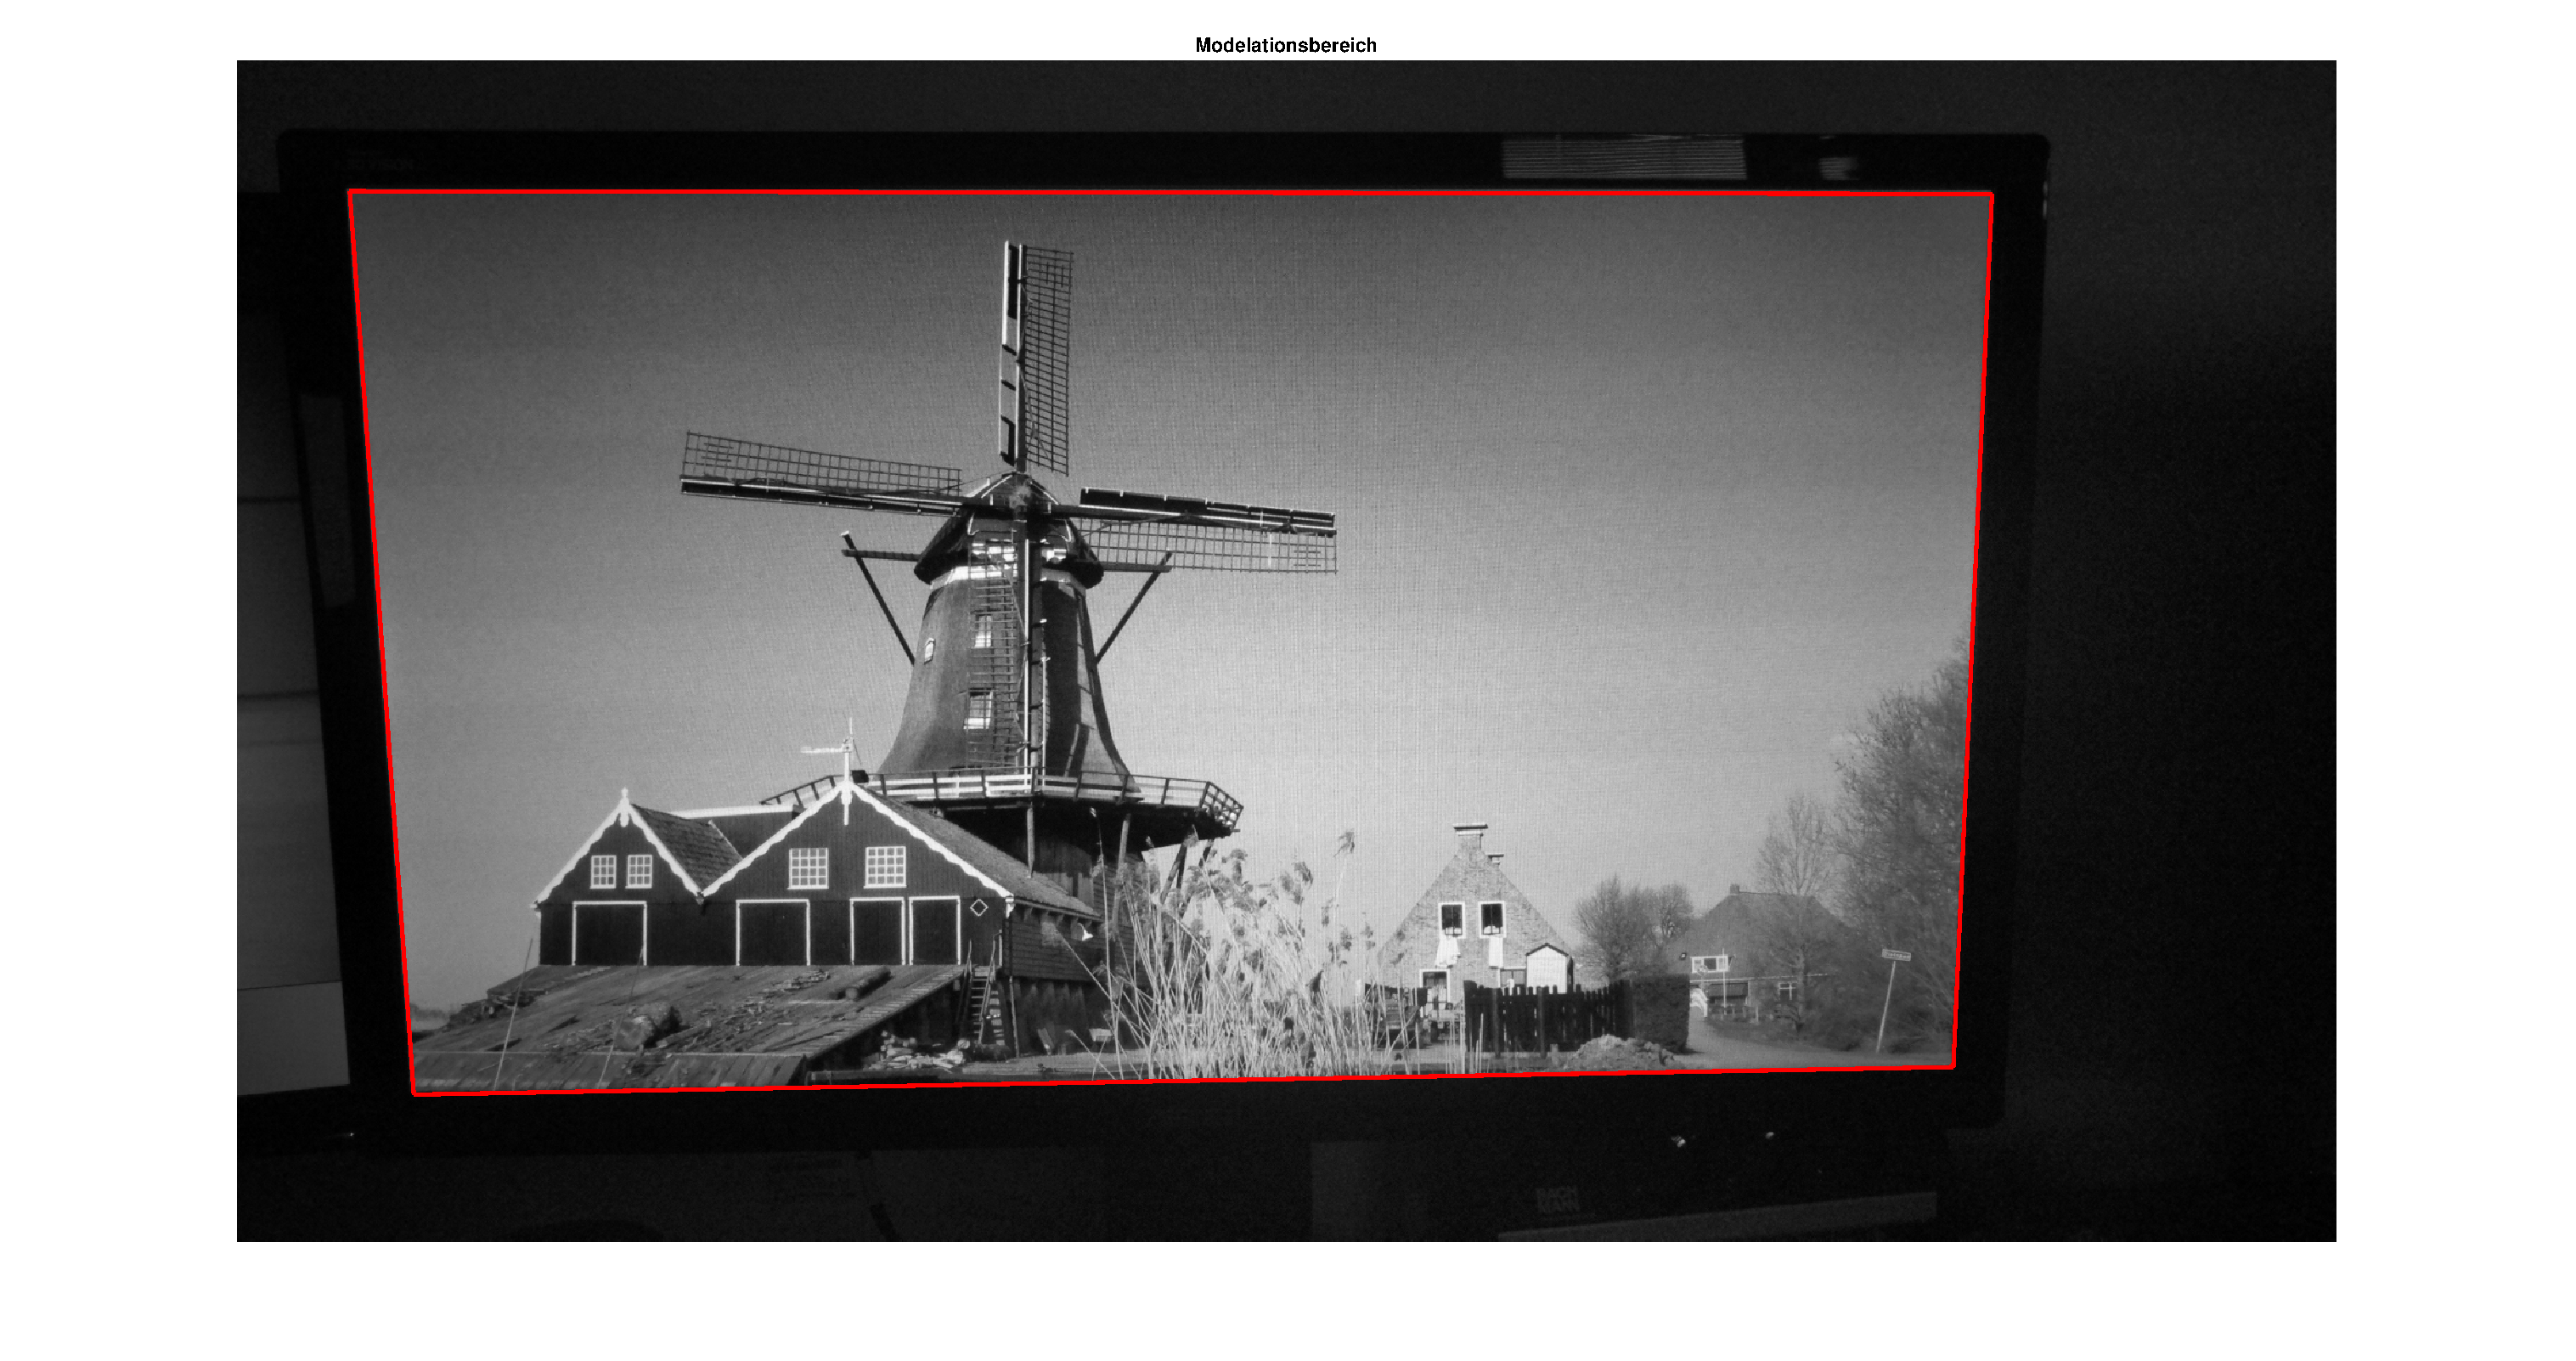
\includegraphics[width=1.0\textwidth]{images/6_Auswertung/Methode1/P1.eps} 
\caption{Cross Dilatation}
\label{fig:cd}
\end{minipage}
\begin{minipage}[b]{0.49\textwidth} 
\centering 
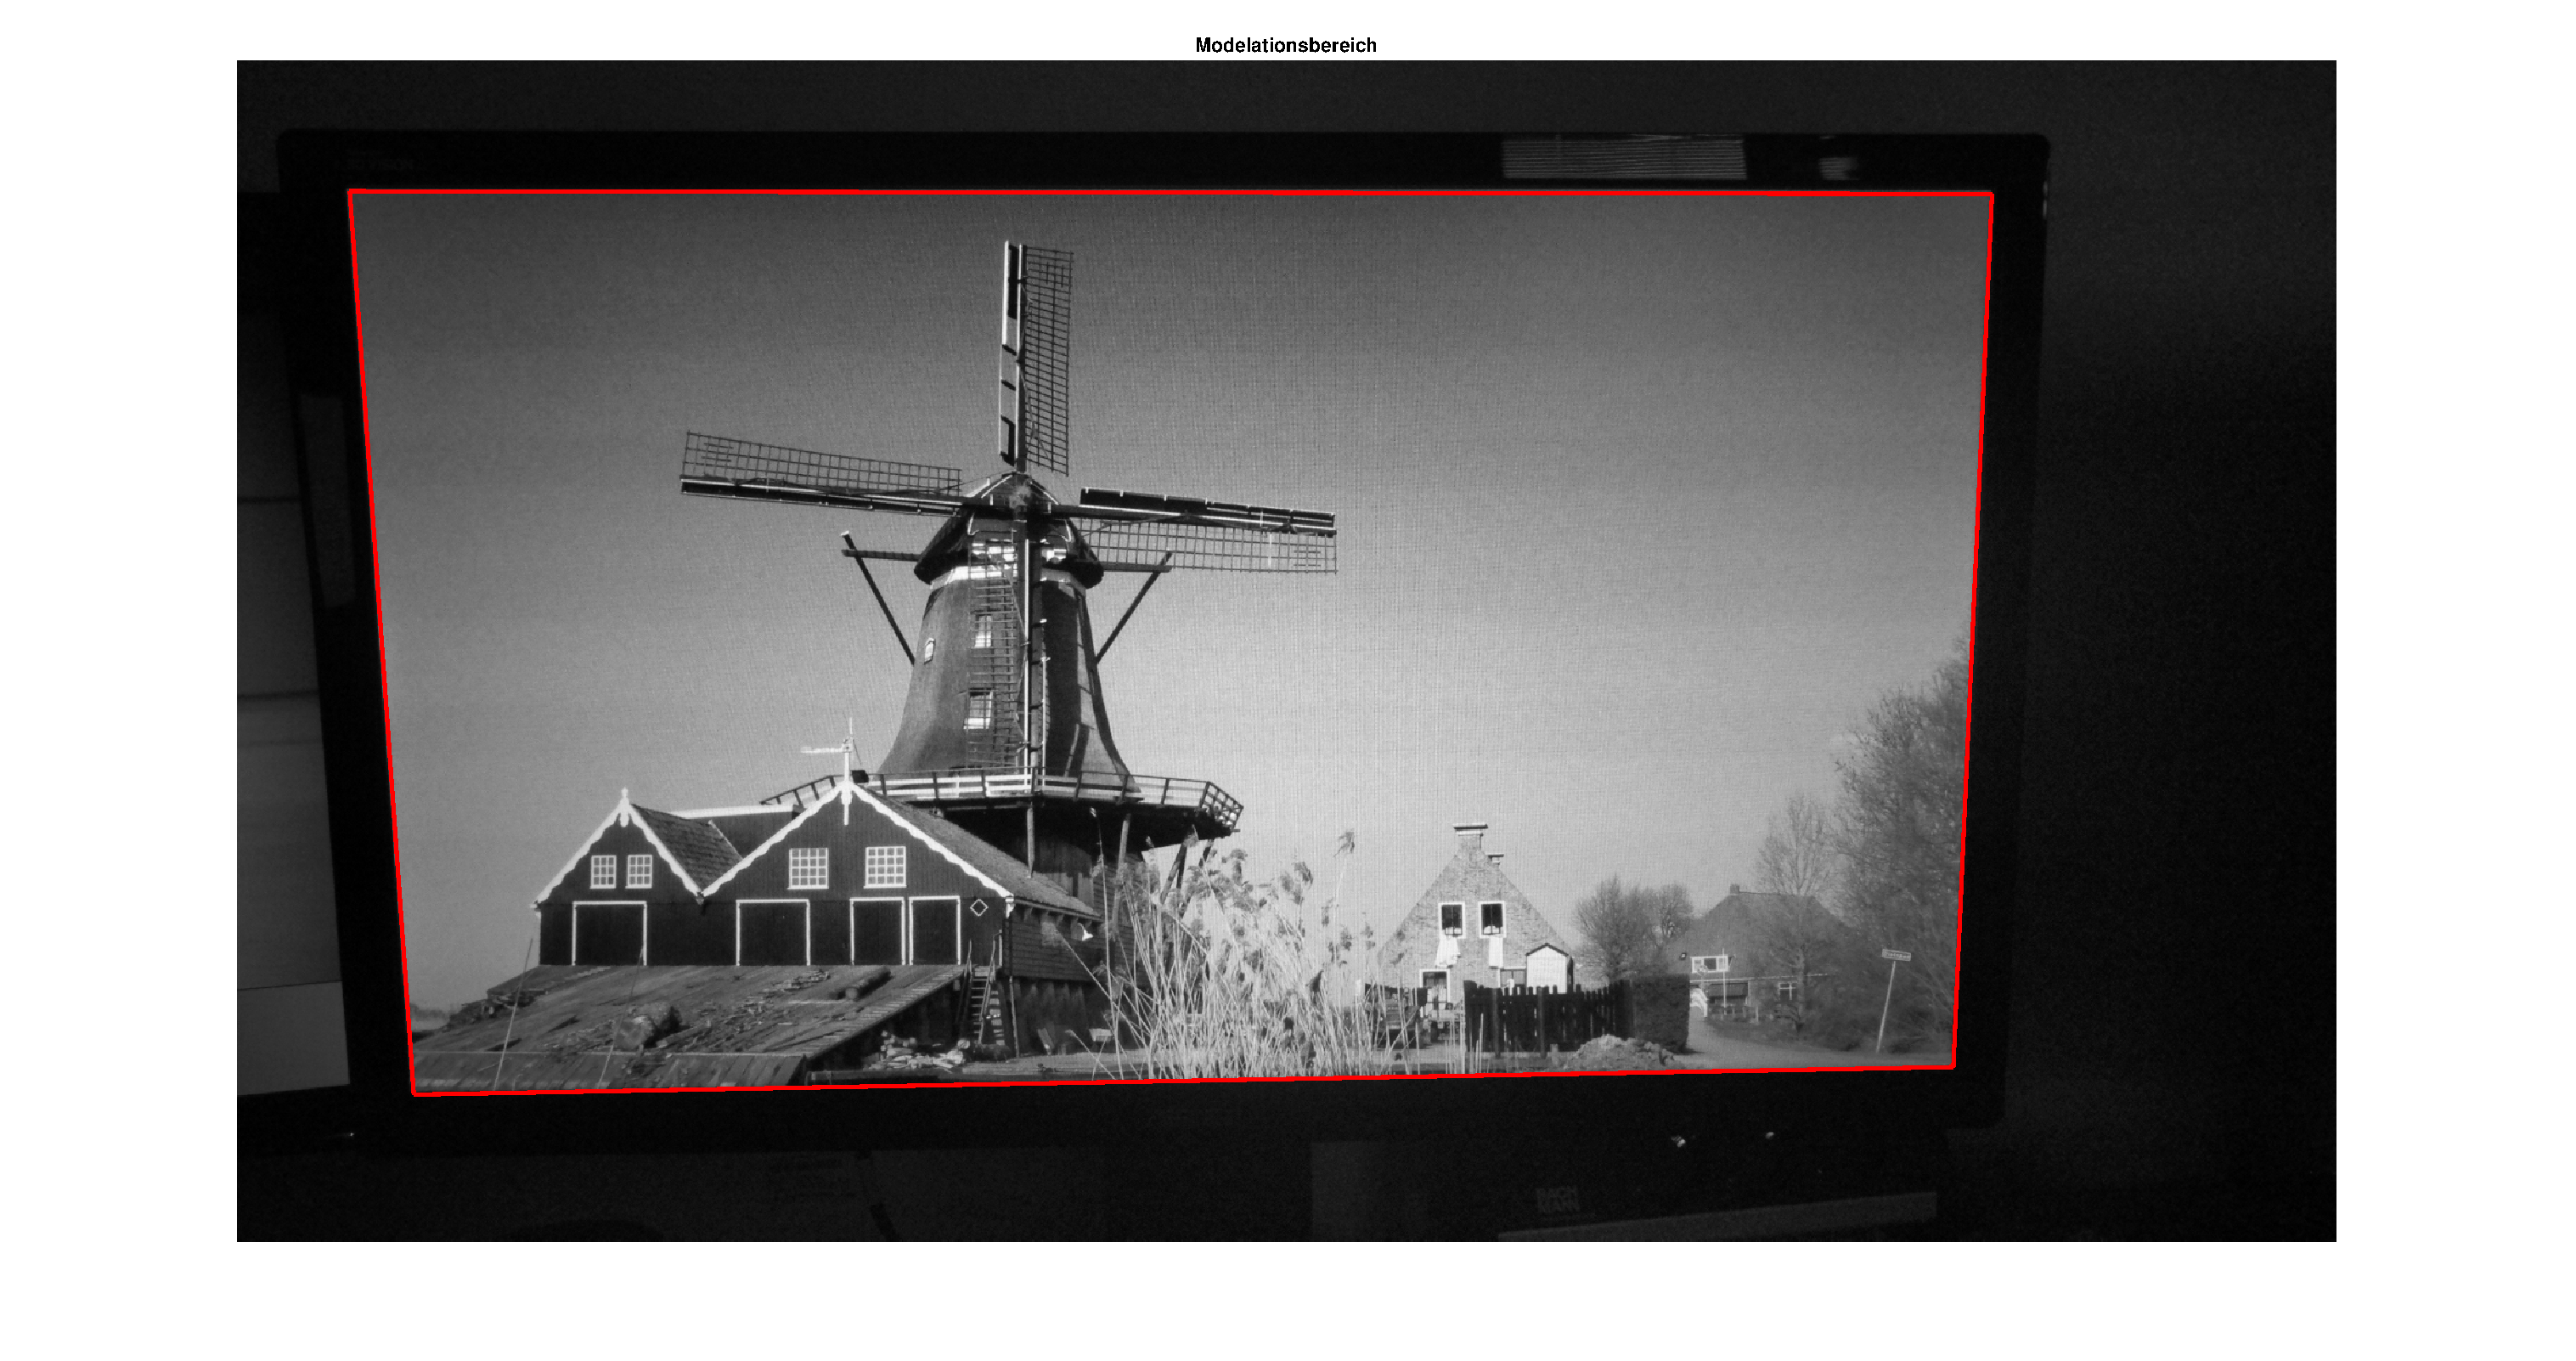
\includegraphics[width=1.0\textwidth]{images/6_Auswertung/Methode1/P1.eps}
\caption{Radon Detektion}
\label{fig:radon}
\end{minipage}
\end{figure}



\section{Evaluierung des 2.Verfahrens}

In diesem Abschnitt wird das 2. Verfahren evaluiert. Wie in Kapitel 4 vorgestellt, ist diese Methode häuptlich für den Fall bei der Aufnahme der Bilder mit einem Smartphone auf einem Stativ. Infolgedessen wird hier die Bildregistrierungs Operation nicht mehr gebraucht. Die Gitterbilder aus dem vorherigen Abschnitt werden hier ebenfalls verwendet. Der Parameter ist eingestellt auf: Modulationsamplitude als 6, der Datenblock als $ 4 \times 4 Pixel$ und die QR Muster Größe als $ 72 \times 72 Pixel $. Die Ergebnisse nach Methode 2 sind in der Abbildung \ref{fig:Ergebnis2} dargestellt.Die berechnete durchschnittliche Abweichung beträgt 1.3468 Pixel. 
\begin{figure}[H]
 \centering 
  \includegraphics[keepaspectratio,width=1.00\textwidth]{images/6_Auswertung/Ergebnis2.pdf}
 \caption{Ergebnis 2}
 \label{fig:Ergebnis2}
\end{figure}